\documentclass{article}

\usepackage{amsmath}
\usepackage{amssymb}
\usepackage{geometry}
\geometry{a4paper, margin=2cm}
\usepackage{xcolor}
\usepackage{tikz}
\usepackage{pgfplots}
\pgfplotsset{compat=1.18}
\usepackage{tcolorbox}
\usepackage{multirow}
\usepackage{array}
\usepackage{booktabs}
\usepackage{hyperref}
\usepackage{colortbl}

% Definición de estilo para los recuadros didácticos
\newtcolorbox{didactico}[1]{%
  colback=blue!5,
  colframe=blue!75!black,
  fonttitle=\bfseries\sffamily,
  title=#1,
  arc=4pt,
  boxrule=1pt,
  left=10pt,
  right=10pt,
  top=8pt,
  bottom=8pt,
  before=\vspace{10pt},
  after=\vspace{10pt}
}

\title{\sffamily\bfseries Guía de Estudio Definitiva: Pruebas de Hipótesis y Medias \\ \large Con Análisis de Errores Tipo I y II, Curvas de Operación C.O. y Dos Medias Poblacionales (Estadística II)}
\author{Tu Profesor Particular de Estadística}
\date{19 de agosto de 2026}

\begin{document}

\maketitle

\tableofcontents
\newpage

\section{Fundamentos de las Pruebas de Hipótesis}

¡Hola! Bienvenido a la versión definitiva y ultra-completa de tu guía de estudio personal. En esta versión, hemos integrado de forma rigurosa todos los gráficos de curvas normales, tablas de decisión, trazados de curvas de operación (C.O.) y las pruebas para comparar dos medias poblacionales, basándonos de manera estricta en las diapositivas y apuntes teóricos de tus clases [1, 2, 7].

\subsection{¿Qué es una hipótesis y una prueba de hipótesis?}

En estadística aplicada, una \textbf{hipótesis} es una suposición sobre un parámetro de la población, como el promedio poblacional $\mu$ [1]. Por ejemplo, podemos suponer que la ganancia promedio de comisión mensual de los vendedores es $\mu = \$2000$ [1]. Dado que sería extremadamente costoso encuestar a toda la población, seleccionamos una \textbf{muestra}, calculamos el promedio muestral ($\bar{x}$) y decidimos si rechazamos o no la hipótesis [1].

Una \textbf{prueba de hipótesis} es el procedimiento estandarizado que nos sirve para decidir si una afirmación sobre un parámetro poblacional es verdadera o falsa, confrontándola con los datos de nuestra muestra [2].

\subsection{La Hipótesis Nula ($H_0$) y la Hipótesis Alternativa ($H_1$)}

\begin{itemize}
    \item \textbf{Hipótesis Nula ($H_0$):} Es nuestro punto de partida. Asumimos temporalmente que es verdadera para confrontarla con los datos [2]. Representa el statu quo. Siempre lleva los signos de igualdad: $=, \le, \ge$ [8, 15].
    \item \textbf{Hipótesis Alternativa ($H_1$ o $H_a$):} Es la hipótesis de investigación [3, 26]. Representa lo que concluimos si la evidencia es suficiente para rechazar $H_0$ [3, 26]. Nunca lleva el signo de igualdad; usa $<, >, \neq$ [8, 15].
\end{itemize}

\begin{didactico}{¿Por qué la hipótesis nula siempre lleva la igualdad?}
Para poder hacer cálculos, necesitamos un valor puntual de referencia ($\mu_0$) sobre el cual centrar nuestra distribución de probabilidad (nuestra campana de Gauss) [2, 13]. La igualdad en $H_0$ nos da ese punto de partida exacto [2, 13]. Si solo dijéramos $\mu > 1600$, tendríamos infinitos valores posibles y no sabríamos dónde colocar el centro de la campana.
\end{didactico}

\section{Guía de Selección: ¿Cuándo usar $Z$ vs. $t$ de Student?}

Una de las decisiones más críticas en los problemas es saber qué distribución usar en base a la población y la muestra. A continuación, se presenta la tabla de resumen basada directamente en tus apuntes, la cual cubre también el uso del \textbf{Teorema de Chebyshev} para poblaciones no normales con muestras pequeñas [18]:

\subsection{Tabla de Selección de Estadísticos e Intervalos}

\begin{table}[h!]
\centering
\small
\renewcommand{\arraystretch}{1.5}
\begin{tabular}{p{3cm} p{3.2cm} p{3.5cm} p{4cm}}
\toprule
\textbf{Población} & \textbf{Tamaño Muestra} & \textbf{$\sigma$ conocida} & \textbf{$\sigma$ desconocida} \\
\midrule
\multirow{2}{=}{\textbf{Normalmente Distribuida}} & Grande ($n \ge 30$) & $\bar{x} \pm z_{\alpha/2} \cdot \sigma_{\bar{x}}$ (Usa $Z$) & $\bar{x} \pm z_{\alpha/2} \cdot s_{\bar{x}}$ (Usa $Z$) \\
\cmidrule{2-4}
& Chica ($n < 30$) & $\bar{x} \pm z_{\alpha/2} \cdot \sigma_{\bar{x}}$ (Usa $Z$) & $\bar{x} \pm t_{\alpha/2} \cdot s_{\bar{x}}$ (Usa $t$ de Student) \\
\midrule
\multirow{2}{=}{\textbf{No Normal o Desconocida}} & Grande ($n \ge 30$) & $\bar{x} \pm z_{\alpha/2} \cdot \sigma_{\bar{x}}$ (Usa $Z$ por TLC) & $\bar{x} \pm z_{\alpha/2} \cdot s_{\bar{x}}$ (Usa $Z$ por TLC) \\
\cmidrule{2-4}
& Chica ($n < 30$) & $\bar{x} \pm k \cdot \sigma_{\bar{x}}$ (Usa Chebyshev) & $\bar{x} \pm k \cdot s_{\bar{x}}$ (Usa Chebyshev) \\
\bottomrule
\end{tabular}
\caption{Tabla de resumen para estimación de intervalos y selección de pruebas para la media [18].}
\end{table}

Donde:
\begin{itemize}
    \item \textbf{TLC (Teorema del Límite Central):} Nos permite asumir que la distribución del promedio muestral se aproxima a una normal si la muestra es grande ($n \ge 30$), incluso si la población original no es normal [18, 20].
    \item \textbf{Teorema de Chebyshev:} Se usa cuando la muestra es chica ($n < 30$) y la población no es normal [18]. Define el intervalo usando una constante $k$ tal que la probabilidad mínima es $1 - 1/k^2$ [18].
\end{itemize}

\section{Anatomía de las Fórmulas Clave}

Estudiemos las fórmulas más importantes con un desglose visual de cada uno de sus componentes:

\subsection{Estadístico de Prueba $Z$ (para una muestra, $\sigma$ conocida)}
\[
z = \frac{ \overbrace{\bar{x}}^{\text{Media muestral}} - \overbrace{\mu_0}^{\text{Media hipotética de referencia}} }{ \underline{\dfrac{\sigma}{\sqrt{n}}} }
\]

\subsection{Estadístico de Prueba $t$ de Student (para una muestra, $\sigma$ desconocida)}
\[
t = \frac{ \overbrace{\bar{x}}^{\text{Media muestral}} - \overbrace{\mu_0}^{\text{Media hipotética de referencia}} }{ \underline{\dfrac{s}{\sqrt{n}}} } \quad \text{con } gl = \underline{n - 1}
\]

\subsection{Límites Críticos de Aceptación (En la escala real de la variable)}
En lugar de transformar la media observada a una escala $z$, podemos calcular las fronteras críticas en las unidades originales del problema (por ejemplo, horas o gramos) [32]:
\[
L_I = \mu_0 - z_{\alpha/2} \cdot s_{\bar{x}} \qquad L_S = \mu_0 + z_{\alpha/2} \cdot s_{\bar{x}}
\]

\newpage
\section{La Regla de Decisión y las Curvas de Probabilidad}

Para tomar una decisión, definimos las regiones de la distribución. A continuación, representamos mediante gráficos nativos de TikZ las tres situaciones típicas:

\subsection{Ensayo Unilateral Derecho (Cola Superior)}
Se utiliza cuando buscamos comprobar un aumento o mejora ($H_a: \mu > \mu_0$) [3, 13]. La región de rechazo se encuentra a la derecha, señalada por la flecha "$>$" de la hipótesis alternativa [13].

\begin{figure}[h!]
\centering
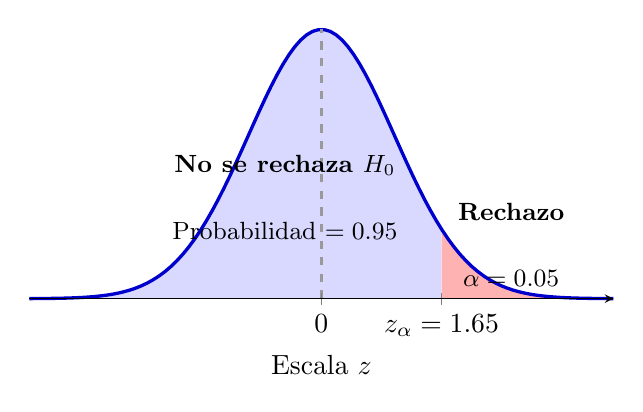
\begin{tikzpicture}
\begin{axis}[
  no markers, domain=-4:4, samples=100,
  axis lines*=left, xlabel={Escala $z$}, ylabel={},
  height=5cm, width=9cm,
  xtick={0, 1.645},
  xticklabels={$0$, $z_{\alpha} = 1.65$},
  ytick=\empty,
  enlargelimits=false, clip=false, axis on top,
  axis x line=bottom, axis y line=none
]
% Zona de No Rechazo (0.95)
\addplot [fill=blue!15, draw=none, domain=-4:1.645] {1/(sqrt(2*3.141592))*exp(-x^2/2)} \closedcycle;
% Cola de Rechazo (0.05)
\addplot [fill=red!30, draw=none, domain=1.645:4] {1/(sqrt(2*3.141592))*exp(-x^2/2)} \closedcycle;
\addplot [very thick, blue!80!black] {1/(sqrt(2*3.141592))*exp(-x^2/2)};
\draw [dashed, thick, black!40] (axis cs:0,0) -- (axis cs:0,0.4);
\node at (axis cs:-0.5, 0.15) [align=center] {\small\textbf{No se rechaza $H_0$}\\\\ \small Probabilidad $= 0.95$};
\node at (axis cs:2.6, 0.08) [align=center] {\small\textbf{Rechazo}\\\\ \small $\alpha = 0.05$};
\end{axis}
\end{tikzpicture}
\caption{Región de rechazo en la cola superior para un ensayo unilateral derecho ($\alpha=0.05$) [13].}
\end{figure}

\subsection{Ensayo Unilateral Izquierdo (Cola Inferior)}
Se utiliza cuando deseamos comprobar una disminución o cuando evaluamos si se cumple una garantía de "por lo menos" ($H_a: \mu < \mu_0$) [5, 6]. El signo de desigualdad "$<$" apunta hacia la cola inferior izquierda [15].

\begin{figure}[h!]
\centering
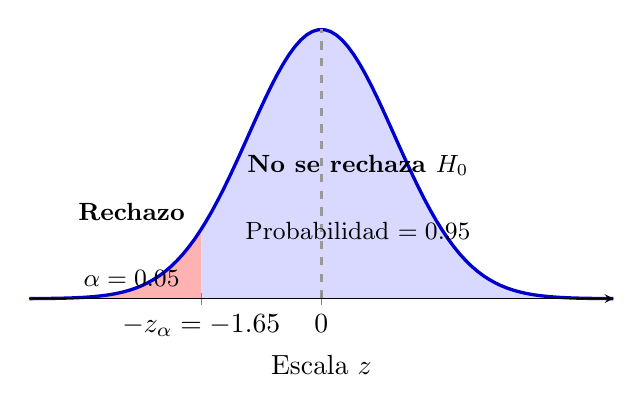
\begin{tikzpicture}
\begin{axis}[
  no markers, domain=-4:4, samples=100,
  axis lines*=left, xlabel={Escala $z$}, ylabel={},
  height=5cm, width=9cm,
  xtick={-1.645, 0},
  xticklabels={$-z_{\alpha} = -1.65$, $0$},
  ytick=\empty,
  enlargelimits=false, clip=false, axis on top,
  axis x line=bottom, axis y line=none
]
% Cola de Rechazo (0.05)
\addplot [fill=red!30, draw=none, domain=-4:-1.645] {1/(sqrt(2*3.141592))*exp(-x^2/2)} \closedcycle;
% Zona de No Rechazo (0.95)
\addplot [fill=blue!15, draw=none, domain=-1.645:4] {1/(sqrt(2*3.141592))*exp(-x^2/2)} \closedcycle;
\addplot [very thick, blue!80!black] {1/(sqrt(2*3.141592))*exp(-x^2/2)};
\draw [dashed, thick, black!40] (axis cs:0,0) -- (axis cs:0,0.4);
\node at (axis cs:0.5, 0.15) [align=center] {\small\textbf{No se rechaza $H_0$}\\\\ \small Probabilidad $= 0.95$};
\node at (axis cs:-2.6, 0.08) [align=center] {\small\textbf{Rechazo}\\\\ \small $\alpha = 0.05$};
\end{axis}
\end{tikzpicture}
\caption{Región de rechazo en la cola inferior para un ensayo unilateral izquierdo ($\alpha=0.05$) [14].}
\end{figure}

\subsection{Ensayo Bilateral (Dos Colas)}
Se utiliza cuando buscamos comprobar si el parámetro ha cambiado o es diferente, sin importar la dirección ($H_a: \mu \neq \mu_0$) [4, 5]. El riesgo $\alpha$ se divide equitativamente entre las dos colas ($\alpha/2$ en cada extremo) [16].

\begin{figure}[h!]
\centering
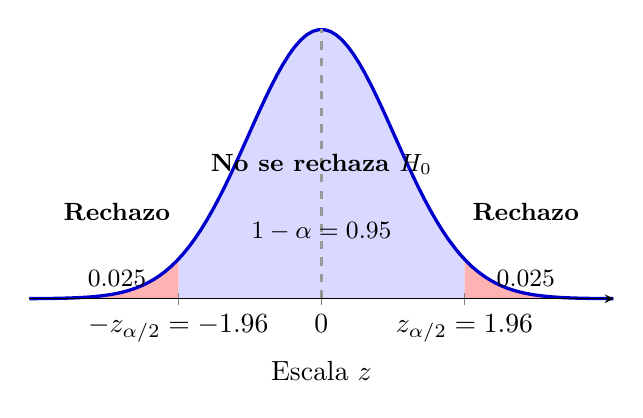
\begin{tikzpicture}
\begin{axis}[
  no markers, domain=-4:4, samples=100,
  axis lines*=left, xlabel={Escala $z$}, ylabel={},
  height=5cm, width=9cm,
  xtick={-1.96, 0, 1.96},
  xticklabels={$-z_{\alpha/2} = -1.96$, $0$, $z_{\alpha/2} = 1.96$},
  ytick=\empty,
  enlargelimits=false, clip=false, axis on top,
  axis x line=bottom, axis y line=none
]
% Zona de No Rechazo (0.95)
\addplot [fill=blue!15, draw=none, domain=-1.96:1.96] {1/(sqrt(2*3.141592))*exp(-x^2/2)} \closedcycle;
% Colas de Rechazo (0.025 cada una)
\addplot [fill=red!30, draw=none, domain=-4:-1.96] {1/(sqrt(2*3.141592))*exp(-x^2/2)} \closedcycle;
\addplot [fill=red!30, draw=none, domain=1.96:4] {1/(sqrt(2*3.141592))*exp(-x^2/2)} \closedcycle;
\addplot [very thick, blue!80!black] {1/(sqrt(2*3.141592))*exp(-x^2/2)};
\draw [dashed, thick, black!40] (axis cs:0,0) -- (axis cs:0,0.4);
\node at (axis cs:0, 0.15) [align=center] {\small\textbf{No se rechaza $H_0$}\\\\ \small $1-\alpha = 0.95$};
\node at (axis cs:-2.8, 0.08) [align=center] {\small\textbf{Rechazo}\\\\ \small $0.025$};
\node at (axis cs:2.8, 0.08) [align=center] {\small\textbf{Rechazo}\\\\ \small $0.025$};
\end{axis}
\end{tikzpicture}
\caption{Distribución muestral en una prueba bilateral ($\alpha=0.05$) con valores críticos correctos ($\pm 1.96$) [16].}
\end{figure}

\begin{didactico}{Aclaración Importante sobre un Error Común en Diapositivas}
En algunas diapositivas de clase se suele ver un gráfico bilateral con $\alpha = 0.05$ donde las colas muestran $\alpha/2 = 0.025$, pero colocan erróneamente el valor de $1.65$ o $-1.65$ en los límites. ¡Ten mucho cuidado!
\begin{itemize}
    \item El valor crítico de \textbf{$1.65$} corresponde a una prueba de \textbf{una sola cola} con un riesgo total $\alpha = 0.05$ [13].
    \item Para una prueba de \textbf{dos colas} con $\alpha = 0.05$, el área de cada cola es $0.025$, lo que nos da valores críticos exactos de \textbf{$\pm 1.96$} [32].
    \item Si la prueba bilateral es con $\alpha = 0.01$ (un nivel del 1\%), entonces el área de cada cola es $0.005$ y los valores críticos son \textbf{$\pm 2.58$} [17, 18].
\end{itemize}
\end{didactico}

\section{¿Cómo buscar valores en la Tabla de Distribución Normal?}

La tabla de distribución normal estándar muestra el área acumulada desde el centro (cero) hacia la derecha [13]. A continuación, te muestro cómo buscar los dos valores más comunes ($1.65$ y $2.58$) simulando los cruces de tu material de clase [14, 18]:

\subsection{Búsqueda del Valor Crítico para Unilateral Derecha ($\alpha = 0.05$)}
Para hallar el valor de $Z$ que deja $0.05$ en la cola superior, restamos $0.05$ a la mitad de la curva ($0.5$): $0.5 - 0.05 = 0.4500$ [13]. Buscamos en el interior de la tabla el valor más cercano a $0.4500$ [13]:

\begin{table}[h!]
\centering
\small
\begin{tabular}{cccccccccc}
\toprule
\textbf{$z$} & \textbf{0.00} & \textbf{0.01} & \textbf{0.02} & \textbf{0.03} & \textbf{0.04} & \cellcolor{red!20}\textbf{0.05} & \textbf{0.06} & \textbf{0.07} & \textbf{0.08} \\
\midrule
1.5 & 0.4332 & 0.4345 & 0.4357 & 0.4370 & 0.4382 & 0.4394 & 0.4406 & 0.4418 & 0.4429 \\
\rowcolor{red!10}
\textbf{1.6} & 0.4452 & 0.4463 & 0.4474 & 0.4484 & 0.4495 & \cellcolor{red!30}\textbf{0.4505} & 0.4515 & 0.4525 & 0.4535 \\
1.7 & 0.4554 & 0.4564 & 0.4573 & 0.4582 & 0.4591 & 0.4599 & 0.4608 & 0.4616 & 0.4625 \\
\bottomrule
\end{tabular}
\caption{Visualización de búsqueda de $z = 1.65$ para un área de $0.4500$ (intersección fila 1.6 y col. 0.05) [14].}
\end{table}

\subsection{Búsqueda del Valor Crítico para Bilateral ($\alpha = 0.01$)}
Para un contraste bilateral con $\alpha = 0.01$, dividimos a la mitad: $\alpha/2 = 0.005$ [17]. Restamos a la mitad de la curva: $0.5 - 0.005 = 0.4950$ [17]. Buscamos el valor más cercano en la tabla [17]:

\begin{table}[h!]
\centering
\small
\begin{tabular}{cccccccccc}
\toprule
\textbf{$z$} & \textbf{0.00} & \textbf{0.01} & \textbf{0.02} & \textbf{0.03} & \textbf{0.04} & \textbf{0.05} & \textbf{0.06} & \textbf{0.07} & \cellcolor{red!20}\textbf{0.08} \\
\midrule
2.4 & 0.4918 & 0.4920 & 0.4922 & 0.4925 & 0.4927 & 0.4929 & 0.4931 & 0.4932 & 0.4934 \\
\rowcolor{red!10}
\textbf{2.5} & 0.4938 & 0.4940 & 0.4941 & 0.4943 & 0.4945 & 0.4946 & 0.4948 & 0.4949 & \cellcolor{red!30}\textbf{0.4951} \\
2.6 & 0.4953 & 0.4955 & 0.4956 & 0.4957 & 0.4959 & 0.4960 & 0.4961 & 0.4962 & 0.4963 \\
\bottomrule
\end{tabular}
\caption{Visualización de búsqueda de $z = 2.58$ para un área de $0.4950$ (intersección de fila 2.5 y col. 0.08) [18].}
\end{table}

\newpage
\section{Análisis de Errores Tipo I y II: El Ejemplo de la Pintura}

Para comprender visualmente cómo interactúan los Errores de Decisión, analizaremos el famoso \textbf{Ejemplo de la Pintura de Secado Rápido} presente en tus diapositivas [1, 2]:

\textbf{Enunciado:} Un fabricante de pintura afirma que su producto seca en un promedio de $\mu = 20$ minutos [1]. Un comprador diseña un experimento: pinta 36 tableros ($n=36$) y decide rechazar el lote si el promedio observado de secado supera los $20.75$ minutos ($\bar{x}_c = 20.75$) [1]. Históricamente se sabe que $\sigma = 2.4$ minutos [2].

Calculamos primero el error estándar de la distribución de medias:
\[
\sigma_{\bar{x}} = \frac{\sigma}{\sqrt{n}} = \frac{2.4}{\sqrt{36}} = 0.4 \text{ minutos}
\]

\subsection{Caso A: El Error Tipo I ($\alpha$)}
¿Cuál es la probabilidad de rechazar la partida (es decir, cometer un Error Tipo I) si la pintura realmente pertenece a una población con media de $\mu_0 = 20$ minutos? [2]

Para calcular la probabilidad de cometer Error Tipo I ($\alpha$), estandarizamos el valor crítico límite de $20.75$ minutos bajo el supuesto de que $\mu_0 = 20$ minutos:
\[
z = \frac{\bar{x}_c - \mu_0}{\sigma_{\bar{x}}} = \frac{20.75 - 20}{0.4} = 1.875
\]

Buscando el área en la tabla de distribución normal hacia la derecha de $z=1.875$:
\[
\alpha = P(Z > 1.875) = 0.5 - 0.4696 = 0.0304 \approx 3\%
\]

Esto significa que hay una probabilidad del \textbf{3.04\%} de rechazar la pintura por puro azar, aun cuando el tiempo promedio real de secado es de $20$ minutos [3].

\begin{figure}[h!]
\centering
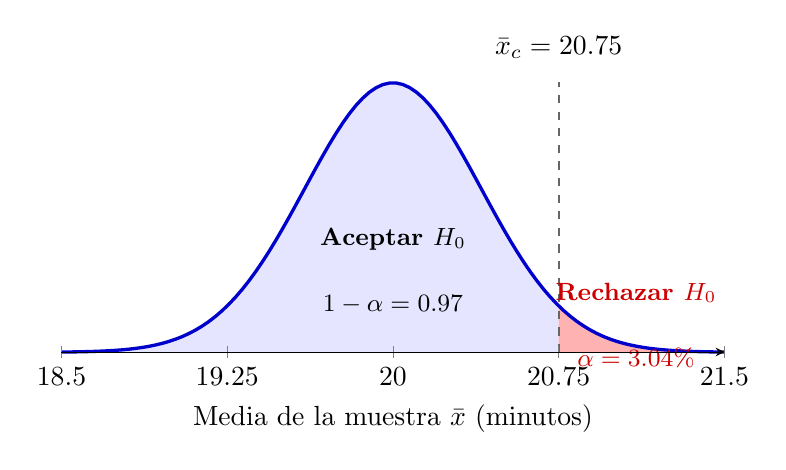
\begin{tikzpicture}
\begin{axis}[
  no markers, domain=18.5:21.5, samples=100,
  axis lines*=left, xlabel={Media de la muestra $\bar{x}$ (minutos)}, ylabel={},
  height=5cm, width=10cm,
  xtick={18.5, 19.25, 20, 20.75, 21.5},
  ytick=\empty,
  enlargelimits=false, clip=false, axis on top,
  axis x line=bottom, axis y line=none
]
  % H0: mean=20, sd=0.4
  \addplot [fill=blue!10, draw=none, domain=18.5:20.75] {1/(0.4*sqrt(2*3.141592))*exp(-(x-20)^2/(2*0.4^2))} \closedcycle;
  \addplot [fill=red!30, draw=none, domain=20.75:21.5] {1/(0.4*sqrt(2*3.141592))*exp(-(x-20)^2/(2*0.4^2))} \closedcycle;
  \addplot [very thick, blue!80!black] {1/(0.4*sqrt(2*3.141592))*exp(-(x-20)^2/(2*0.4^2))};
  \draw [dashed, thick, black!60] (axis cs:20.75,0) -- (axis cs:20.75,1.0);
  \node at (axis cs:20.75, 1.05) [above] {$\bar{x}_c = 20.75$};
  \node at (axis cs:20, 0.3) [align=center] {\small\textbf{Aceptar $H_0$}\\\\ \small $1-\alpha = 0.97$}; 
  \node at (axis cs:21.1, 0.1) [align=center, red!80!black] {\small\textbf{Rechazar $H_0$}\\\\ \small $\alpha = 3.04\%$};
\end{axis}
\end{tikzpicture}
\caption{Distribución de medias bajo $H_0$ ($\mu_0 = 20$) mostrando la probabilidad de cometer Error Tipo I ($\alpha = 0.0304$) [2].}
\end{figure}

\subsection{Caso B: El Error Tipo II ($\beta$)}
Supongamos ahora que la pintura es defectuosa y su media real es de $\mu = 21$ minutos [3]. ¿Cuál es la probabilidad de que nuestra prueba acepte erróneamente el lote (cometiendo un Error Tipo II)? [3]

Para calcular $\beta$, evaluamos la probabilidad de que el promedio de las muestras sea menor o igual a $20.75$ minutos, calculando bajo el supuesto de la curva real defectuosa ($\mu = 21$):
\[
z = \frac{\bar{x}_c - \mu}{\sigma_{\bar{x}}} = \frac{20.75 - 21}{0.4} = -0.625
\]

El área hacia la izquierda de $z=-0.625$ en la curva normal estándar es:
\[
\beta = P(Z \le -0.625) = 0.5 - 0.2340 = 0.2660 \approx 26.6\%
\]

Es decir, si la pintura seca en promedio en 21 minutos, existe un \textbf{26.6\%} de probabilidad de cometer un falso negativo y aceptarla como buena por puro error de muestreo [4].

\begin{figure}[h!]
\centering
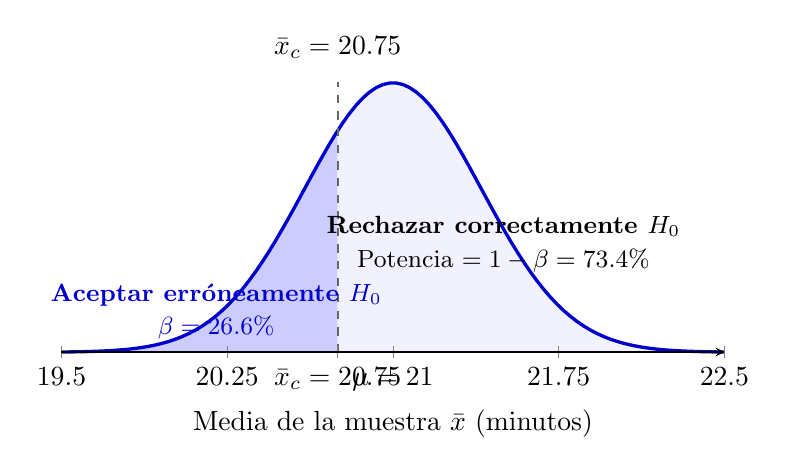
\begin{tikzpicture}
\begin{axis}[
  no markers, domain=19.5:22.5, samples=100,
  axis lines*=left, xlabel={Media de la muestra $\bar{x}$ (minutos)}, ylabel={},
  height=5cm, width=10cm,
  xtick={19.5, 20.25, 20.75, 21, 21.75, 22.5},
  xticklabels={$19.5$, $20.25$, $\bar{x}_c=20.75$, $\mu=21$, $21.75$, $22.5$},
  ytick=\empty,
  enlargelimits=false, clip=false, axis on top,
  axis x line=bottom, axis y line=none
]
  % H1: mean=21, sd=0.4
  \addplot [fill=blue!20, draw=none, domain=19.5:20.75] {1/(0.4*sqrt(2*3.141592))*exp(-(x-21)^2/(2*0.4^2))} \closedcycle;
  \addplot [fill=blue!5, draw=none, domain=20.75:22.5] {1/(0.4*sqrt(2*3.141592))*exp(-(x-21)^2/(2*0.4^2))} \closedcycle;
  \addplot [very thick, blue!80!black] {1/(0.4*sqrt(2*3.141592))*exp(-(x-21)^2/(2*0.4^2))};
  \draw [dashed, thick, black!60] (axis cs:20.75,0) -- (axis cs:20.75,1.0);
  \node at (axis cs:20.75, 1.05) [above] {$\bar{x}_c = 20.75$};
  \node at (axis cs:20.2, 0.15) [align=center, blue!80!black] {\small\textbf{Aceptar erróneamente $H_0$}\\ \small $\beta = 26.6\%$};
  \node at (axis cs:21.5, 0.4) [align=center] {\small\textbf{Rechazar correctamente $H_0$}\\ \small Potencia $= 1-\beta = 73.4\%$};
\end{axis}
\end{tikzpicture}
\caption{Distribución de medias bajo $H_1$ ($\mu = 21$) mostrando la probabilidad de cometer Error Tipo II ($\beta = 0.2660$) [4].}
\end{figure}

\newpage
\subsection{El Gráfico Definitivo: Interacción de Ambos Errores (Curvas Superpuestas)}

Si superponemos ambas curvas, podemos apreciar con absoluta claridad de qué manera el límite de decisión $\bar{x}_c = 20.75$ actúa como un divisor exacto de áreas. 
Si movemos la línea hacia la izquierda para achicar $\beta$, el área roja ($\alpha$) aumenta; si la movemos hacia la derecha para achicar $\alpha$, el área azul ($\beta$) crece [8]. Esta es la tensión fundamental de las pruebas de hipótesis [8].

\begin{figure}[h!]
\centering
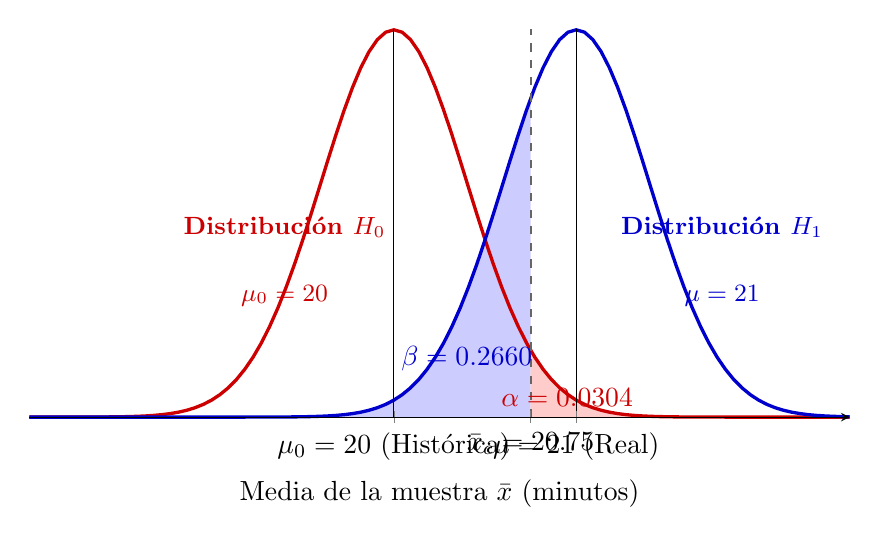
\begin{tikzpicture}
\begin{axis}[
  no markers, domain=18:22.5, samples=100,
  axis lines*=left, xlabel={Media de la muestra $\bar{x}$ (minutos)}, ylabel={},
  height=6.5cm, width=12cm,
  xtick={20, 20.75, 21},
  xticklabels={$\mu_0=20$ (Histórica), $\bar{x}_c=20.75$, $\mu=21$ (Real)}, 
  ytick=\empty,
  enlargelimits=false, clip=false, axis on top,
  axis x line=bottom, axis y line=none
]
  % Shade beta under curve centered at 21 (blue curve) to the left of 20.75
  \addplot [fill=blue!20, draw=none, domain=18:20.75] {1/(0.4*sqrt(2*3.141592))*exp(-(x-21)^2/(2*0.4^2))} \closedcycle;
  % Shade alpha under curve centered at 20 (red curve) to the right of 20.75
  \addplot [fill=red!20, draw=none, domain=20.75:22.5] {1/(0.4*sqrt(2*3.141592))*exp(-(x-20)^2/(2*0.4^2))} \closedcycle;
  
  % Plot H0 curve
  \addplot [very thick, red!80!black] {1/(0.4*sqrt(2*3.141592))*exp(-(x-20)^2/(2*0.4^2))};
  % Plot H1 curve
  \addplot [very thick, blue!80!black] {1/(0.4*sqrt(2*3.141592))*exp(-(x-21)^2/(2*0.4^2))};
  
  \draw [dashed, thick, black!60] (axis cs:20.75,0) -- (axis cs:20.75,1.0);
  \draw (axis cs:20,0) -- (axis cs:20,1.0);
  \draw (axis cs:21,0) -- (axis cs:21,1.0);
  
  \node at (axis cs:19.4, 0.4) [red!80!black, align=center] {\small\textbf{Distribución $H_0$}\\\\ \small $\mu_0 = 20$};
  \node at (axis cs:21.8, 0.4) [blue!80!black, align=center] {\small\textbf{Distribución $H_1$}\\\\ \small $\mu = 21$};
  
  \node at (axis cs:20.4, 0.15) [blue!80!black] {$\beta = 0.2660$};
  \node at (axis cs:20.95, 0.05) [red!80!black] {$\alpha = 0.0304$};
\end{axis}
\end{tikzpicture}
\caption{Interacción de Errores Tipo I ($\alpha$) y II ($\beta$) representados mediante curvas normales superpuestas [20].}
\end{figure}

\begin{didactico}{¿Por qué no fijamos siempre un alfa extremadamente pequeño?}
Al achicar la región de rechazo de forma artificial (mover el límite a la derecha en este gráfico), reducimos la probabilidad del Error Tipo I ($\alpha$). Pero observa lo que le sucede al área azul: ¡se agranda drásticamente!
Por lo tanto, al disminuir $\alpha$ aumentamos de manera inevitable la probabilidad de cometer Error Tipo II ($\beta$), lo que significa perder potencia en la prueba para detectar cambios reales [8].

La única forma matemáticamente válida para reducir ambos errores de forma simultánea es \textbf{aumentar el tamaño de la muestra ($n$)}, ya que esto comprime las campanas de Gauss hacia el centro y encoge ambas regiones de error simultáneamente [26].
\end{didactico}


\subsection{Estudio de Impacto Real: Contraste Práctico de Errores Tipo I y II (Envasadora de Café)}

Para complementar tu preparación ante el tribunal oral, analizaremos de forma práctica qué significan y qué consecuencias tienen el Error Tipo I ($\alpha$) y el Error Tipo II ($\beta$) utilizando el ejemplo de la **máquina envasadora de café en bolsas de 500 gramos** ($n = 36$, $\sigma_{\bar{x}} = 2$ gramos, $\alpha = 0.05$).

\subsubsection{Caso A: Escenario de Cola Derecha (Sobrellenado)}
\begin{itemize}
    \item \textbf{Límite de Decisión ($x_{crit}$):} $503.29$ gramos.
    \item \textbf{Error Tipo I ($\alpha = 5\%$):} La máquina está perfectamente calibrada ($\mu = 500$g), pero por puro azar, la muestra da un promedio de $504$g. Detienes la planta y pagas mantenimiento sin necesidad. Es una \textbf{falsa alarma}.
    \item \textbf{Error Tipo II ($\beta = 19.5\%$):} La máquina está rota y regala café ($\mu = 505$g), pero por azar del muestreo, la muestra da un promedio de $502$g. No haces nada, creyendo que todo funciona bien. Es una \textbf{pérdida económica invisible e ineficiente}.
\end{itemize}

\subsubsection{Caso B: Escenario de Cola Izquierda (Subllenado)}
\begin{itemize}
    \item \textbf{Límite de Decisión ($x_{crit}$):} $496.71$ gramos.
    \item \textbf{Error Tipo I ($\alpha = 5\%$):} La máquina llena bien ($500$g), pero la muestra da un promedio de $495$g. Detienes la producción acusando falsamente al proceso de subllenado. Es un \textbf{conflicto y costo innecesario}.
    \item \textbf{Error Tipo II ($\beta = 19.5\%$):} La máquina está rota y estafa al cliente ($\mu = 495$g), pero la muestra da un promedio de $498$g. No haces nada, asumiendo que todo está normal. Es un \textbf{riesgo legal gravísimo (clausuras y multas)}.
\end{itemize}

\subsubsection{Caso C: Escenario Bilateral de Dos Colas (Descalibración)}
\begin{itemize}
    \item \textbf{Límites de Decisión ($L_I, L_S$):} $[496.08\text{ g}, 503.92\text{ g}]$.
    \item \textbf{Error Tipo I ($\alpha = 5\%$):} La máquina está perfecta ($500$g), pero la muestra da un promedio de $504.2$g. Detienes la planta para recalibrar un sistema que funcionaba de forma idónea.
    \item \textbf{Error Tipo II ($\beta = 29.5\%$):} La máquina está descalibrada a $505$g, pero la muestra da un promedio de $502.5$g. Asumes que está bien calibrada e ignoras el desajuste, perpetuando la pérdida de materia prima.
\end{itemize}

\begin{table}[h!]
\centering
\small
\renewcommand{\arraystretch}{1.5}
\begin{tabular}{p{2.8cm} p{4.6cm} p{4.6cm}}
\toprule
\textbf{Escenario} & \textbf{Error Tipo I ($\alpha = 5\%$)} & \textbf{Error Tipo II ($\beta$)} \\
\midrule
\textbf{Cola Derecha} \newline (Sobrellenado) & 
\textbf{Falsa Alarma:} \newline 
La máquina llena a $500$g pero la muestra da $504$g. Detienes la planta y pagas mantenimiento sin necesidad. & 
\textbf{Pérdida Silenciosa:} \newline 
La máquina llena a $505$g pero la muestra da $502$g. No haces nada y sigues regalando café. \\
\midrule
\textbf{Cola Izquierda} \newline (Subllenado) & 
\textbf{Falsa Alarma:} \newline 
La máquina está perfecta ($500$g) pero la muestra da $495$g. Haces una falsa acusación de fraude. & 
\textbf{Riesgo de Multa:} \newline 
La máquina estafa con $495$g pero la muestra da $498$g. No detectas el subllenado y te arriesgas a multas del estado. \\
\midrule
\textbf{Dos Colas} \newline (Descalibración) & 
\textbf{Falsa Alarma:} \newline 
La máquina está calibrada a $500$g pero la muestra da $504.2$g. Desajustas un sistema que funcionaba bien. & 
\textbf{Ineficiencia:} \newline 
La máquina está desviada a $505$g pero la muestra da $502.5$g. Asumes que está bien calibrada e ignoras el fallo. \\
\bottomrule
\end{tabular}
\caption{Matriz de impacto práctico de los errores de decisión en la planta de café.}
\end{table}

\begin{didactico}{El Mensaje que debes dar al Tribunal Oral}
``Señores profesores, el Error Tipo I ($\alpha$) representa el costo de la \textbf{impaciencia y las falsas alarmas} (intervenir un proceso que está sano); mientras que el Error Tipo II ($\beta$) representa el costo de la \textbf{ceguera y la ineficiencia} (dejar correr un proceso que está dañado). Ambas probabilidades están unidas por un cordón umbilical: si intentamos reducir la probabilidad de falsas alarmas haciendo el rango de aceptación más estricto, aumentamos inmediatamente el riesgo de quedarnos ciegos ante descalibraciones reales.''
\end{didactico}

\section{Curvas Características de Operación (C.O.) y su Trazado}

La probabilidad de aceptar la hipótesis nula ($L(\mu)$ o $\beta$) varía de forma continua para cada valor real posible que tome la media de la población [17]. La curva característica de operación representa gráficamente esta probabilidad en el eje de ordenadas frente a los posibles valores del parámetro poblacional real en abscisas [17, 18].

\subsection{Matemáticas del Trazado de la Curva C.O.}

Para trazar las curvas C.O. de forma matemática, se define la variable $d$ (discrepancia estandarizada) como el tamaño del efecto [28]:
\[
d = \frac{|\mu - \mu_0|}{\sigma}
\]

Para un contraste unilateral derecho con significación $\alpha = 0.05$ ($z_\alpha = 1.645$) and una muestra de tamaño $n$, la función que describe la probabilidad de cometer Error Tipo II es [28]:
\[
\beta(d, n) = 0.5 + \int_{0}^{1.645 - d\sqrt{n}} \frac{1}{\sqrt{2\pi}} \exp(-0.5x^2) dx
\]

En un entorno de simulación y gráficos (como MATLAB o R), esta integral se modela para distintos valores de $n$, obteniendo curvas que se hacen cada vez más pendientes a medida que $n$ aumenta [28, 29].

\begin{figure}[h!]
\centering
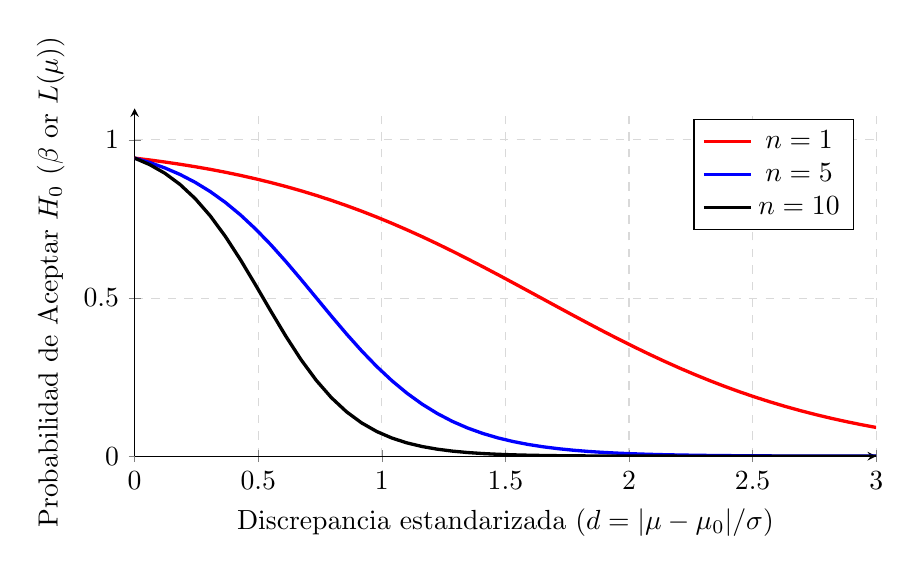
\begin{tikzpicture}
\begin{axis}[
  domain=0:3, samples=50,
  axis lines=left, 
  xlabel={Discrepancia estandarizada ($d = |\mu-\mu_0|/\sigma$)},
  ylabel={Probabilidad de Aceptar $H_0$ ($\beta$ or $L(\mu)$)},
  height=6cm, width=11cm,
  ymin=0, ymax=1.1, xmin=0, xmax=3,
  legend pos=north east,
  grid=both, grid style={dashed, gray!30}
]
% Curva para n=1
\addplot [very thick, red] {1 / (1 + exp(-1.7 * (1.645 - x * sqrt(1))))};
\addlegendentry{$n=1$}
% Curva para n=5
\addplot [very thick, blue] {1 / (1 + exp(-1.7 * (1.645 - x * sqrt(5))))};
\addlegendentry{$n=5$}
% Curva para n=10
\addplot [very thick, black] {1 / (1 + exp(-1.7 * (1.645 - x * sqrt(10))))};
\addlegendentry{$n=10$}
\end{axis}
\end{tikzpicture}
\caption{Curvas Características de Operación (C.O.) para tres tamaños muestrales distintos (Unilateral) [29].}
\end{figure}

\subsection{Código MATLAB para Trazar las Curvas C.O.}

A continuación, se muestra el bloque de código de MATLAB presente en tus diapositivas, que permite calcular y trazar de forma exacta las tres curvas del gráfico superior [28]:

\begin{tcolorbox}[colback=black!5, colframe=black!70, fonttitle=\bfseries\sffamily, title=Función de Trazado Matlab]
\begin{verbatim}
function curvas_ope
% Expresion de la funcion densidad normal
F=inline('1/sqrt(2*pi)*exp(-0.5*x.^2)');

% Generacion de la curva para n=1
n=1; i=1; 
for d=0:0.1:3
    M1(i)=0.5+quadl(F,0,1.65-d*sqrt(n)); i=i+1;
end

% Generacion de la curva para n=5
n=5; i=1;
for d=0:0.1:3
    M2(i)=0.5+quadl(F,0,1.65-d*sqrt(n)); i=i+1;
end

% Generacion de la curva para n=10
n=10; i=1;
for d=0:0.1:3
    M3(i)=0.5+quadl(F,0,1.65-d*sqrt(n)); i=i+1;
end

a=i-1; i=1:a;
plot(i, M1, 'r', i, M2, 'b', i, M3, 'k')

% El gráfico generado muestra a n=1 (rojo, superior),
% n=5 (azul, central) y n=10 (negro, inferior).
\end{verbatim}
\end{tcolorbox}

\newpage
\section{Pruebas de Hipótesis para Dos Medias Poblacionales}

En muchas aplicaciones prácticas, no comparamos un promedio contra un estándar rígido, sino que comparamos los promedios de dos poblaciones distintas ($\mu_1$ y $\mu_2$) [34]. La hipótesis nula suele afirmar que no existen diferencias significativas entre ellas: $H_0: \mu_1 - \mu_2 = \delta$ (donde comúnmente $\delta = 0$, implicando $\mu_1 = \mu_2$) [35, 37].

\subsection{Caso 1: Muestras Independientes, Varianzas Conocidas o Muestras Grandes}
Si conocemos las desviaciones estándar de ambas poblaciones ($\sigma_1, \sigma_2$) o si las muestras independientes son grandes ($n_1 \ge 30, n_2 \ge 30$) de modo que estimamos con las desviaciones típicas muestrales ($s_1, s_2$) [36]:

\subsubsection*{Anatomía del Estadístico $Z$ Bimuestral}
\[
z = \frac{ \overbrace{(\bar{x}_1 - \bar{x}_2)}^{\text{Diferencia promedio observada}} - \overbrace{\delta}^{\text{Diferencia poblacional supuesta bajo } H_0} }{ \sqrt{\dfrac{\sigma_1^2}{n_1} + \dfrac{\sigma_2^2}{n_2}} }
\]

\subsubsection*{Ejemplo Práctico 1: Resistencia de Conductores Eléctricos y Aleación}
\textbf{Enunciado:} Para probar si la resistencia media de un conductor eléctrico puede reducirse en más de $0.050$ ohms al añadir una aleación, se toman 32 muestras sin aleación ($\bar{x}_1 = 0.136$ ohms, $s_1 = 0.004$ ohms) y 32 muestras con aleación ($\bar{x}_2 = 0.083$ ohms, $s_2 = 0.005$ ohms) [37]. ¿Se apoya la afirmación con $\alpha = 0.05$? [37]

\begin{enumerate}
    \item \textbf{Paso 1: Hipótesis.} $H_0: \mu_1 - \mu_2 = 0.050$ ohms vs. $H_a: \mu_1 - \mu_2 > 0.050$ ohms (unilateral derecha) [38].
    \item \textbf{Paso 2: Significancia.} $\alpha = 0.05 \Rightarrow z_{crit} = 1.65$ [38].
    \item \textbf{Paso 3: Cálculos.} Como las muestras son de gran tamaño ($32 \ge 30$), aproximamos usando $s_1$ y $s_2$ [36]:
    \[
    z_{calc} = \frac{(0.136 - 0.083) - 0.050}{\sqrt{\dfrac{0.004^2}{32} + \dfrac{0.005^2}{32}}} = \frac{0.003}{\sqrt{0.0000005 + 0.000000781}} = \frac{0.003}{0.00113} \approx 2.65
    \]
    \item \textbf{Paso 4: Regla de decisión.} Rechazamos $H_0$ si $z_{calc} > 1.65$ [37].
    \item \textbf{Paso 5: Conclusión.} Como $2.65 > 1.65$, rechazamos rotundamente $H_0$ [38]. El alambre con aleación reduce significativamente la resistencia eléctrica en más de $0.050$ ohms [38].
\end{enumerate}

\subsection{Caso 2: Muestras Independientes, Varianzas Desconocidas pero Iguales, Muestras Pequeñas}
Si no conocemos las desviaciones estándar poblacionales, pero suponemos que son idénticas ($\sigma_1^2 = \sigma_2^2$), agrupamos nuestras variaciones para calcular la \textbf{Varianza Agrupada o Ponderada ($s_p^2$)} [42]:

\subsubsection*{Anatomía del Estadístico $t$ Bimuestral}
\[
s_p^2 = \frac{ \overbrace{(n_1 - 1)s_1^2}^{\text{Suma de cuadrados Grupo 1}} + \overbrace{(n_2 - 1)s_2^2}^{\text{Suma de cuadrados Grupo 2}} }{ n_1 + n_2 - 2 }
\]
\[
t = \frac{ \overbrace{(\bar{x}_1 - \bar{x}_2)}^{\text{Diferencia promedios}} - \overbrace{\delta}^{\text{Diferencia supuesta}} }{ \sqrt{s_p^2 \left(\dfrac{1}{n_1} + \dfrac{1}{n_2}\right)} } \quad \text{con } \nu = n_1 + n_2 - 2
\]

\subsubsection*{Ejemplo Práctico 2: Incremento en Producción de Trigo (Fertilizante)}
\textbf{Enunciado:} Una estación agrícola ensaya un fertilizante en 24 parcelas ($n_1=n_2=12$) [43]. Las no tratadas rinden $\bar{x}_2 = 0.264\text{ m}^3$ con $s_2 = 0.02\text{ m}^3$ y las tratadas rinden $\bar{x}_1 = 0.28\text{ m}^3$ con $s_1 = 0.022\text{ m}^3$ [43]. ¿Sube significativamente la producción al $\alpha = 0.05$? [43]

\begin{enumerate}
    \item \textbf{Paso 1: Hipótesis.} $H_0: \mu_1 - \mu_2 = 0$ (no hay diferencia) vs. $H_a: \mu_1 - \mu_2 > 0$ (incremento de trigo) [44].
    \item \textbf{Paso 2: Significancia y grados de libertad.} $\alpha = 0.05$ y $\nu = 12 + 12 - 2 = 22 \Rightarrow t_{crit} = 1.717$ [44].
    \item \textbf{Paso 3: Cálculos.}
    \[ s_p^2 = \frac{11 \cdot (0.022)^2 + 11 \cdot (0.02)^2}{22} = 0.000442 \]
    \[ t_{calc} = \frac{0.28 - 0.264}{\sqrt{0.000442 \left(\dfrac{2}{12}\right)}} = \frac{0.016}{0.00858} \approx 1.849 \]
    \item \textbf{Paso 4: Regla.} Rechazar $H_0$ si $t_{calc} > 1.717$ [44].
    \item \textbf{Paso 5: Decisión.} Como $1.849 > 1.717$, rechazamos $H_0$. El uso de fertilizante incrementa significativamente la producción de trigo [45].
\end{enumerate}

\subsection{Caso 3: Muestras Apareadas (Estudios de Antes y Después)}
Cuando las dos mediciones no son independientes sino que pertenecen a los mismos sujetos (estudios de antes-después o gemelos) [45], analizamos la diferencia individual con su respectivo signo $d_i = x_{1i} - x_{2i}$ [45]. Esto convierte el problema en una prueba $t$ de una sola muestra para la diferencia [46]:

\subsubsection*{Anatomía del Estadístico $t$ Apareado}
\[
t = \frac{ \overbrace{\bar{d}}^{\text{Promedio muestral de diferencias}} - \overbrace{\mu_d}^{\text{Diferencia esperada (habitualmente 0)}} }{ \dfrac{s_d}{\sqrt{n}} } \quad \text{con } gl = n - 1
\]

\subsubsection*{Ejemplo Práctico 3: Horas-Hombre Perdidas por Accidentes}
\textbf{Enunciado:} Diez plantas industriales miden accidentes semanales antes ($X_1$) y después ($X_2$) de implantar un plan de seguridad:

Antes: $45, 73, 46, 124, 33, 57, 83, 34, 26, 17$ [45].\\
Después: $36, 60, 44, 119, 35, 51, 77, 29, 24, 11$ [45].\\
Evaluar si el plan de seguridad es eficaz con un nivel $\alpha = 0.05$ [45].

\begin{enumerate}
    \item \textbf{Paso 1: Hipótesis.} Calculamos las diferencias individuales $d_i = \text{Antes} - \text{Después}$:
    \[ d_i = \{9, 13, 2, 5, -2, 6, 6, 5, 2, 6\} \]
    Si el programa es eficaz, se deben reducir los accidentes (es decir, $Antes > Despues$), por lo que planteamos [46]:
    \[ H_0: \mu_d = 0 \qquad H_a: \mu_d > 0 \text{ (unilateral de cola derecha)} \]
    \item \textbf{Paso 2: Significancia y grados de libertad.} $\alpha = 0.05$ y $\nu = 10 - 1 = 9 \Rightarrow t_{crit} = 1.833$ [46].
    \item \textbf{Paso 3: Cálculos.} Calculamos el promedio y desviación de la muestra de diferencias:
    \[ \bar{d} = 5.2 \text{ horas}, \quad s_d = 4.077 \text{ horas} \]
    \[ t_{calc} = \frac{5.2 - 0}{4.077/\sqrt{10}} = 4.033 \]
    \item \textbf{Paso 4: Regla.} Rechazar $H_0$ si $t_{calc} > 1.833$ [46].
    \item \textbf{Paso 5: Conclusión.} Como $4.033 > 1.833$, rechazamos de forma abrumadora la hipótesis nula. El programa de seguridad es eficaz para reducir los accidentes [47].
\end{enumerate}

\begin{didactico}{¿Por qué las diferencias eliminan el sesgo de la planta?}
Si utilizáramos la prueba bimuestral común, estaríamos ignorando que la medición ``después'' pertenece a la misma planta que la medición ``antes'' [45]. El nivel base de accidentes varía enormemente de una planta a otra. Al calcular la diferencia individual $d_i$ de cada planta, cancelamos de un plumazo esa variabilidad inicial de fondo, permitiendo que la prueba enfoque toda su atención únicamente en el verdadero cambio provocado por el programa de seguridad.
\end{didactico}

\newpage
\subsection{Curva C.O. para la Diferencia de Dos Medias (Ejemplo de Estaturas)}

¿Sabías que también podemos calcular el Error Tipo II ($\beta$) al comparar dos medias? Esto depende directamente del tamaño de las muestras y de la diferencia real alterna $\delta'$ entre las poblaciones [40].

\textbf{Ejemplo del Resumen Definitivo [38, 40]:} Se ensaya si los estudiantes que participan en pruebas atléticas tienen una estatura promedio superior a los que no participan, con un $\alpha = 0.05$ [38]. Muestras de $n_1=n_2=50$ estudiantes revelan:

Grupo atlético: $\bar{x}_1 = 1.70$ mts, $s_1 = 0.0625$ mts [38].\\
Grupo de control: $\bar{x}_2 = 1.687$ mts, $s_2 = 0.07$ mts [38].

Se quiere saber la probabilidad de cometer Error Tipo II ($\beta$) para una diferencia real de estaturas de $\delta' = 0.02$ metros [40].

\textbf{Cálculo del Estadístico de Discrepancia d:} 
\[
d = \frac{|\delta - \delta'|}{\sqrt{\sigma_1^2 + \sigma_2^2}} = \frac{|0 - 0.02|}{\sqrt{0.0625^2 + 0.07^2}} = \frac{0.02}{0.0938} = 0.213 \text{ metros}
\]

Al ejecutar el algoritmo en MATLAB (o R) para calcular $\beta$ en una prueba unilateral con $n=50$ y $d=0.213$:
\[
\beta = \text{error\_II}(1, 0.05, 0, 0.02, \sigma, 50) = 0.5549
\]

Esto significa que la probabilidad de cometer Error Tipo II es del \textbf{55.49\%} [41], lo que refleja un alto riesgo de equivocarse (aceptar que no hay diferencias cuando la diferencia real de estaturas es de $2$ cm). El p-valor se ubica en $z_{calc} = 0.98 < 1.65$, concluyendo originalmente que no se puede rechazar la hipótesis nula [40].

\begin{figure}[h!]
\centering
\begin{tikzpicture}
\begin{axis}[
  domain=0:1, samples=50,
  axis lines=left, 
  xlabel={Discrepancia d ($\delta'$)}, 
  ylabel={Probabilidad de Aceptar $H_0$ ($\beta$)},
  height=5.5cm, width=10cm,
  xtick={0, 0.213, 0.5, 1.0},
  xticklabels={$0$, $d=0.213$, $0.5$, $1.0$},
  ytick={0, 0.5549, 1},
  yticklabels={$0$, $\beta=0.555$, $1$},
  ymin=0, ymax=1.1, xmin=0, xmax=1,
  grid=both, grid style={dashed, gray!30}]
\end{axis}
\end{tikzpicture}
\caption{Curva C.O. para la diferencia de dos medias en el ejemplo de estaturas ($n=50$).}
\end{figure}

\newpage
\section{Ejemplos Resueltos de una Sola Media Poblacional}

A continuación se resuelven paso a paso tres ejemplos reales aplicando rigurosamente los 5 pasos oficiales [2]:

\subsection{Ejemplo A: Duración de Bombillas LED ($Z$, Unilateral)}
\textbf{Problema:} $\sigma = 500$ horas, $\mu = 10,000$ horas históricas [19, 20]. Una muestra de $n = 40$ bombillas rinde un promedio de $\bar{x} = 10,200$ horas [20]. Evaluar al $\alpha = 0.05$.

\begin{enumerate}
    \item \textbf{Paso 1: Plantear hipótesis.} $H_0: \mu \le 10,000$ vs. $H_a: \mu > 10,000$ (cola derecha, pues buscamos comprobar aumento) [14].
    \item \textbf{Paso 2: Significancia.} $\alpha = 0.05$.
    \item \textbf{Paso 3: Estadístico de prueba.} Como $\sigma$ es conocida y $n \ge 30$, usamos $Z$ [20]:
    \[ z_{calc} = \frac{10,200 - 10,000}{500/\sqrt{40}} = 2.53 \]
    \item \textbf{Paso 4: Regla de decisión.} Al ser unilateral derecho con $\alpha=0.05$, el valor crítico es $z_{crit} = 1.65$ [14]. Rechazamos $H_0$ si $z_{calc} > 1.65$ [14].
    \item \textbf{Paso 5: Decisión.} Como $2.53 > 1.65$, se rechaza $H_0$. El nuevo filamento aumenta significativamente la vida útil promedio de las bombillas LED [21].
\end{enumerate}

\subsection{Ejemplo B: Producción de Escritorios Modelo A325 ($Z$, Bilateral)}
\textbf{Enunciado:} Una empresa fabrica y arma escritorios de oficina. La producción semanal del modelo A325 tiene una distribución normal con una media histórica de $\mu = 200$ y una desviación estándar de $\sigma = 16$. Tras introducir nuevos métodos de producción y contratar más empleados, se quiere investigar si hubo algún cambio en la cantidad media de escritorios producidos por semana. Para un nivel de significancia de $\alpha = 0.01$ y una muestra de $n = 50$ semanas con un promedio observado de $\bar{x} = 203.5$, tomar la decisión.

\begin{figure}[h!]
\centering
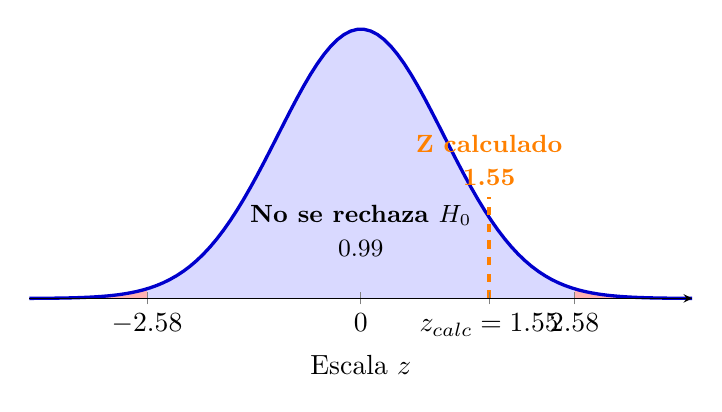
\begin{tikzpicture}
\begin{axis}[
  no markers, domain=-4:4, samples=100,
  axis lines*=left, xlabel={Escala $z$}, ylabel={},
  height=5cm, width=10cm,
  xtick={-2.58, 0, 1.55, 2.58},
  xticklabels={$-2.58$, $0$, $z_{calc} = 1.55$, $2.58$},
  ytick=\empty,
  enlargelimits=false, clip=false, axis on top,
  axis x line=bottom, axis y line=none
]
% Zona de No Rechazo (0.99)
\addplot [fill=blue!15, draw=none, domain=-2.58:2.58] {1/(sqrt(2*3.141592))*exp(-x^2/2)} \closedcycle;
% Colas de Rechazo (0.005)
\addplot [fill=red!30, draw=none, domain=-4:-2.58] {1/(sqrt(2*3.141592))*exp(-x^2/2)} \closedcycle;
\addplot [fill=red!30, draw=none, domain=2.58:4] {1/(sqrt(2*3.141592))*exp(-x^2/2)} \closedcycle;
\addplot [very thick, blue!80!black] {1/(sqrt(2*3.141592))*exp(-x^2/2)};
% Línea de nuestro estadístico calculado
\draw [dashed, ultra thick, orange] (axis cs:1.55,0) -- (axis cs:1.55,0.15) node[above, orange, align=center] {\small\textbf{Z calculado}\\\small\textbf{1.55}};
\node at (axis cs:0, 0.1) [align=center] {\small\textbf{No se rechaza $H_0$}\\\small $0.99$};
\end{axis}
\end{tikzpicture}
\caption{Visualización gráfica de la prueba bilateral de escritorios Modelo A325 ($\alpha = 0.01$).}
\end{figure}

\begin{enumerate}
    \item \textbf{Paso 1: Plantear hipótesis.} Queremos comprobar si la producción es diferente de 200:
    \[ H_0: \mu = 200 \qquad H_a: \mu \neq 200 \]
    \item \textbf{Paso 2: Significancia.} $\alpha = 0.01$. Al ser bilateral, cada cola tiene un área de $\alpha/2 = 0.005$ [17].
    \item \textbf{Paso 3: Estadístico de prueba.} Conocemos $\sigma = 16$ y la muestra es grande ($n = 50 \ge 30$). Usamos $Z$:
    \[ z_{calc} = \frac{\bar{x} - \mu}{\sigma/\sqrt{n}} = \frac{203.5 - 200}{16/\sqrt{50}} = \frac{3.5}{2.2627} \approx 1.55 \]
    \item \textbf{Paso 4: Regla de decisión.} Los valores críticos para $\alpha/2 = 0.005$ son $\pm 2.58$ [18]. No rechazamos $H_0$ si $-2.58 \le z_{calc} \le 2.58$.\\
    \item \textbf{Paso 5: Decisión.} Nuestro valor $z_{calc} = 1.55$ cae cómodamente dentro de la \textbf{Región de No Rechazo} (pues $-2.58 \le 1.55 \le 2.58$).
\end{enumerate}

\textbf{Significado en lenguaje cotidiano:} No rechazamos $H_0$. No hay evidencia suficiente al 1\% de significancia para afirmar que la cantidad promedio de escritorios producidos ha cambiado. La diferencia entre el promedio observado ($203.5$) y el promedio histórico ($200$) puede atribuirse razonablemente al azar de la muestra.

\subsection{Ejemplo C: Tubos Fluorescentes (Límites Críticos, Cola Izquierda)}
\textbf{Problema:} Probar si el promedio difiere de $1600$ horas para una muestra de $n = 100$, $\bar{x} = 1570$ horas y $s = 120$ horas con $\alpha = 0.05$ utilizando límites críticos [27].

\begin{enumerate}
    \item \textbf{Paso 1: Hipótesis.} $H_0: \mu = 1600$ hs vs. $H_a: \mu \neq 1600$ hs [28].
    \item \textbf{Paso 2: Error estándar.} $s_{\\bar{x}} = s/\sqrt{n} = 120/\sqrt{100} = 12$ hs [31].\\
    \item \textbf{Paso 3: Límites críticos.} Para $\alpha = 0.05$ bilateral, los cuantiles son $z_{\alpha/2} = \pm 1.96$ [32].
    \[ L_I = 1600 - 1.96 \cdot 12 = 1576.48 \text{ hs} \qquad L_S = 1600 + 1.96 \cdot 12 = 1623.52 \text{ hs} \]
    \item \textbf{Paso 4: Regla de decisión.} No se rechaza $H_0$ si el promedio de la muestra $\bar{x}$ está en el intervalo de aceptación $[1576.48, 1623.52]$ hs [33].
    \item \textbf{Paso 5: Conclusión.} Como $\bar{x} = 1570 < L_I$ ($1570 < 1576.48$), rechazamos $H_0$ [40].
\end{enumerate}

\textbf{Significado en lenguaje cotidiano:} La muestra cae en la zona de rechazo (cola izquierda) [40]. Concluimos que la duración media real de todos los tubos es significativamente distinta de 1600 horas (de hecho, es inferior) [41]. La compañía debe inspeccionar la línea de fabricación [41].

\end{document}